\section{Przeprowadzone eksperymenty} \label{results}


\subsection{Sztuczne powiekszanie zbioru danych}
\subsubsection{Opis problemu}
Eksperyment sztucznego powiększania danych został przeprowadzony w opraciu o konkurs ,,Dogs vs. Cats'' opublikowanego w serwisie Kaggle.\footnotemark Zadaniem uczestników było stworzenie systemu, który jest w stanie rozwiązać problem rozpoznawania psów i kotów na obrazie. Udostępnione zostało baza danych 25000 sklasyfikowanych obrazów o różnych rozmiarach. Mały wycinek udostępnionych danych został przedstawiony na rysunku \ref{catsdogs}. W celu ewaluacji i otrzymania wyniku wykorzystywany był zbiór 12500 niesklasyfikowanych obrazów. Najlepsze rezultaty uczestnicy otrzymywali przy użyciu głębokich sieci neuronów i także ta metoda została wykorzystana w tej pracy.Zwyciezca pierwszej edycji konkursu uzyskal skutecznosc 98,9\%\footnotemark korzystajac wlasnie z glebokich sieci neuronowych.Celem tego eksperymentu było zbadania poprawy klasyfikacji przy użyciu sztucznego powielania danych. Najprosciej ujmujac, cale postepowanie mozna opisac w dwoch krokach. Pierwszym z nich jest uczenie przy uzyciu oryginalnych obrazow. Drugim natomiast, uczenie przy wykorzystywaniu lekko zmodyfikowanych obrazow. W kroku drugim jednak, mozna rowniez wyszczegolnic dwa podejscia:
\begin{itemize}
\item statyczne powielanie obrazow,
\item dynamiczne powielanie obrazow.
\end{itemize}
Stayczne generowanie obrazow polega na stworzeniu ich przed uruchomieniem programu. Mozna okreslic liczbe obrazow, ktore chcemy stworzyc dla kazdego obrazu oryginalnego, nastepnie wygenerowac docelowe obrazy aby ostatecznie uzyc ich do uczenia sieci neuronowej. W przypadku dynamicznego generowanie obrazow, jest ono wykonywane w trakcie dzialania programu za kazdym razem gdy siec potrzebuje danych. Przy uwzglednieniu wystarczajacej ilosci zmiennych losowych zapewnia to, ze z bardzo duzym prawdopodbienstwem nie zostana wykorzystane do uczenia dokladnie dwa takie same obrazy.
\footnotetext{\url{https://www.kaggle.com/c/dogs-vs-cats}}
\footnotetext{\url{https://plus.google.com/+PierreSermanet/posts/GxZHEH9ynoj}}

\begin{figure}[ht!]
\centering
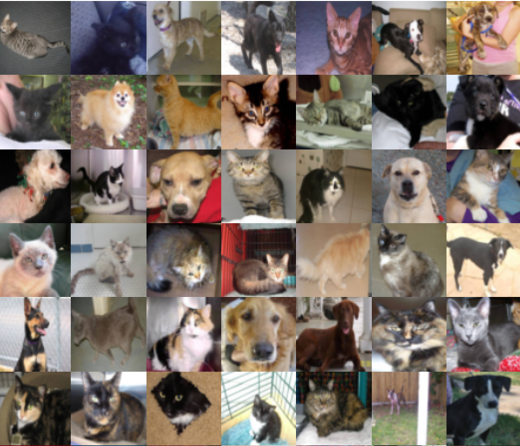
\includegraphics[scale=0.8]{res/catsdogs.png}
\caption[Caption for LOF]{Przykładowe zdjęcia z bazy danych serwisu Kaggle dla konkursu ,,Dogs vs. Cats'' \label{catsdogs}}
\end{figure} 

\subsubsection{Stworzone rozwiązanie}
System stworzony w przypadku tego eksperymentu składał się z dwóch głównych komponentów. W celu wyodrębnienia wczytywania oraz generowania danych stworzony został komponent nazwany DataProvider, który pozwalał w zręczny sposób podawać dane do sieci. Drugim komponentem była sama sieć neuronowa. Ze względy jednak na duże wymogi obliczeniowe w przypadku uczenia, możliwości dobrania odpowiedniej architektury oraz optymalizowania parametrów były dość ograniczone. Pojedyncze uczenie sieci, wraz z ewaluacją trwało około 17 godzin. Dla uzyskania statystyki, ze względu na zmienne losowe występujące w tej metodzie, uczenie przeprowadzane było w każdym przypadku 5 razy. Wszystkie wykorzystywane obrazy zostały zmniejszony do rozmiarów 64x64. Ostatecznie dobrana architektura sieci zawierała trzy warstwy konwolucyjne, jedną warstwę typu \textit{max pooling}, jedną warstwę w pełni połączoną (\textit{fully connected}) tj. taką, która występuję w tradycyjnej sieci neuronowej oraz jedną warstwę wyjściową. Warstwa wyjściowa składała się z dwóch neuronów odpowiednio dla dwóch rozpoznawanych na obrazach klas. W przypadku warstw konwolucyjnych, wszystkie posiadały po 64 filtry z tym, że w pierwszych dwóch stosowana była maska o rozmiarach 7x7, a w trzeciej 5x5.  Warstwa w pełni połączona zawierała 512 neuronów.
\subsubsection{Wyniki}
W tabeli \ref{table:catdogs} przedstawione zostały wyniki dla sieci uruchamianej przy wykorzystaniu sztucznego powielania cech oraz bez użycia tej techniki. Czy powinienem tutaj jeszcze dodac jakies wyniki? Można przedstawić tutaj wykresy pokazujące skuteczność w zależności od iteracji dla obu przypadków, ale wydaje mi się, że nic to nie wnosi.

\begin{table}
\centering
\begin{tabular}{|c|c|}
\hline
Skuteczność uzyskany przy wykorzystaniu sztucznego powielania danych & $72\% \pm 2\%$ \\
\hline 
Skuteczność uzyskana bez wykorzystania sztucznego powielania danych & $69\% \pm 1\%$ \\
\hline 
 \end{tabular}
 \caption{Porównanie wyników z zastosowaniem metody sztucznego powielania danych} \label{table:catdogs}
\end{table}

\subsubsection{Wnioski}

\subsection{Walidacja krzyżowa}
\subsubsection{Opis problemu}
W tym podrozdziale autor starał się porównać podejście z wykorzystaniem walidacji krzyżowej oraz tradycyjne podzielenie zbioru danych na zbiór uczący, testowy oraz walidacyjny. Przeprowadzona została kolejno optymalizacja parametrów dla czterech algorytmów tj. maszyna wektorów nośnych, sztuczne sieci neuronowe, las drzew decyzyjnych oraz pojedyncze drzewo decyzyjne. W każdym przypadku optymalizacja parametrów modelu została przeprowadzona za pomocą metody walidacji krzyżowej oraz wg tradycyjnego podejścia.  Algorytmy były testowane na sztucznie wygenerowanych zbiorze zawierającym 7 atrybutów oraz różną ilość danych. Następnie porównane zostały wyniki dla parametrów wyznaczonych wg obu metod dla wszystkich testowanych algorytmów
\subsubsection{Wyniki}
\subsubsection{Wnioski}

\subsection{Ekstrakcja cech przy użyciu metod matematycznych}

\subsubsection{Opis problemu}
Matematycznymi metodami wykorzystanymi do ekstrakcji cech danych były analiza głównych składowych oraz liniowa analiza dyskryminacyjna. Przetestowane zostały cztery algorytmy uczenia maszynowego tj. maszyna wektorów nośnych, sztuczne sieci neuronowe, las drzew decyzyjnych oraz pojedyncze drzewo decyzyjne. Wykorzystanym zbiorem danych był zbiór o nazwie \textit{digits} dostępny w bibliotece scikit-learn. Posiada on 64 atrybuty. Obliczenia przeprowadzone zostały na liczbie danych wynoszącej kolejno 300 oraz 600. Zmniejszana była kolejno liczba atrybutów aż do momentu, gdy zbiór posiadał jeden atrybut. W każdym przypadku przeprowadzane były obliczenia w celu określenia skuteczności danej metody na zbiorze danych po zastosowaniu na nim ekstrakcji cech w celu określenia czy operacja ta pomaga w otrzymaniu wyższej skuteczności.

\subsubsection{Stworzony rozwiązanie}
\subsubsection{Wyniki}
\subsubsection{Wnioski}

\subsection{Ekstrakcja cech przy użyciu ,,wiedzy''}
\subsubsection{Opis problemu}
W niniejszym podrozdziale rozważanym zagadnieniem była ekstrakcja cech przy użyciu ,,wiedzy'' polegająca transformacji danych do przestrzeni o mniejszej wymiarowości przy wykorzystaniu wiedzy, którą posiadamy na temat naszych danych. Pomysł na ten eksperyment został zaczerpnięty z \cite{higgs1}. Wykorzystane zostały także dane opisane w artykule, które są danymi zebranymi z detektorów cząstek ulokowanych w Wielkim Zderzaczu Hadronów (\textit{Large Hadron Collider}, LHC) będącym największym na świecie akceleratorem cząstek, który ulokowany jest w Europejskim Ośrodku Badań Jądrowych CERN w pobliżu Genewy. Głównym celem działania LHC jest zgłębienie wiedzy na temat cząstek elementarnych. W celu izolacji sygnału od tła w przypadku posiadania danych z odpowiednich detektorów szeroko wykorzystywane jest uczenie maszynowe. Artykuł opisuje wykorzystanie głębokich sieci neuronowych dla problemu wyodrębnienia cząstki Higgsa. Udostępnione dane zawierają 11 milionów rekordów dla których określonych jest 21 cech fizycznych tzw. niskiego poziomu. Każdy rekord opisany jest także za pomocą 7 atrybutów wysokiego poziomu, które obliczone zostały na podstawie cech niskiego poziomu. Celem obliczeń było zobrazowanie faktu, iż poniżej pewnej ilości danych, użycie głębokich sieci neuronowych nie przynosi tak spektakularnych rezultatów oraz użycie ekstrakcji cech może znacznie poprawić wyniki. Obok głębokiej sieci neuronowej, wykorzystane zostały algorytmy takiej jak tradycyjne sieć neuronowa, las drzew decyzyjnych oraz pojedyncze drzewo decyzyjne.

\subsubsection{Stworzone rozwiązanie}
Stworzony program składał się z dwóch głównych komponentów. Pierwszym z nich był komponent o nazwie HiggsModels, który służył do stworzenia odpowiedniej głębokiej sieci neuronowej w zależności od używanych atrybutów. Drugim natomiast, Optimizer, który odpowiadał za odpowiednią optymalizacje parametrów dla tradycyjnych algorytmów uczenia maszynowego.

\subsubsection{Wyniki}
\subsubsection{Wnioski}

